\documentclass[aspectratio=169,grey,smaller]{beamer}
\usetheme{Singapore}
\usecolortheme{seagull}

\usepackage[T1]{fontenc}
\usepackage[utf8]{inputenc}
\usepackage{german}
\usepackage{graphicx}
\usepackage{array}
\usepackage{hhline}
\usepackage{color}
\usepackage{lmodern}
\usepackage{listings}
\usepackage{scrextend}
\lstset{basicstyle=\ttfamily,breaklines=true}
\graphicspath{{./pictures/}}

\title{Elastic Beanstalk}
\date{3. November 2017}
\author{Gregor Bückendorf}

\begin{document}

\begin{frame}
  \titlepage
\end{frame}

\section{Grundlagen}
\subsection{}

\begin{frame}
  \frametitle{Was ist Elastic Beanstalk?}
  \begin{itemize}
  \item<2-> Ein Weg für Anwendungsentwickler Webapps hochverfügbar in die Amazon Cloud zu bringen, ohne sich um Resources kümmern zu müssen
  \item<3-> Ein Werkzeug zum verwalten von Deployment Environments in der Amazon Cloud
  \item<4-> 4 AWS Resource Types
  \end{itemize}
\end{frame}

\begin{frame}
  \frametitle{Die Application}
  \framesubtitle{AWS::ElasticBeanstalk::Application}
  \begin{columns}
  \begin{column}{.48\textwidth}
  \begin{itemize}
  \item<2-> Ein Container für Application Versions
  \item<3-> Regeln zur automatischen Löschung alter Versionen
  \end{itemize}
  \end{column}
  \begin{column}{.48\textwidth}
  \begin{flushright}
  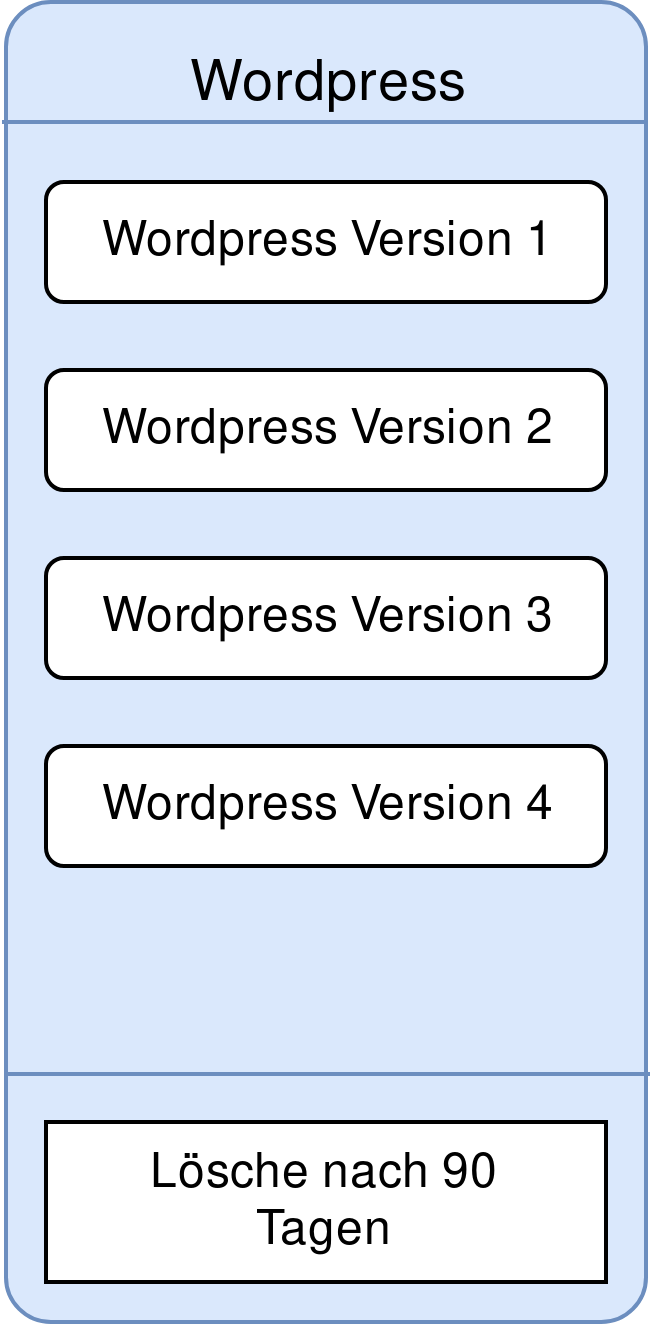
\includegraphics[height=5.5cm]{application}
  \end{flushright}
  \end{column}
  \end{columns}
\end{frame}

\begin{frame}
  \frametitle{Die Version}
  \framesubtitle{AWS::ElasticBeanstalk::ApplicationVersion}
  \begin{columns}
  \begin{column}{.48\textwidth}
  \uncover<1->{Ein Link zu einem Objekt in einem S3-Bucket}
  \begin{itemize}
  \item<2-> wird hier Sourcebundle genannt
  \item<3-> ist meistens eine .zip-Datei
  \item<4-> enthält die eigentliche Applikation \uncover<5->{( z.B. den Inhalt von /var/www/html )}
  \item<6-> kann auch Konfigurationen enthalten
  \end{itemize}
  \end{column}
  \begin{column}{.48\textwidth}
  \begin{flushright}
  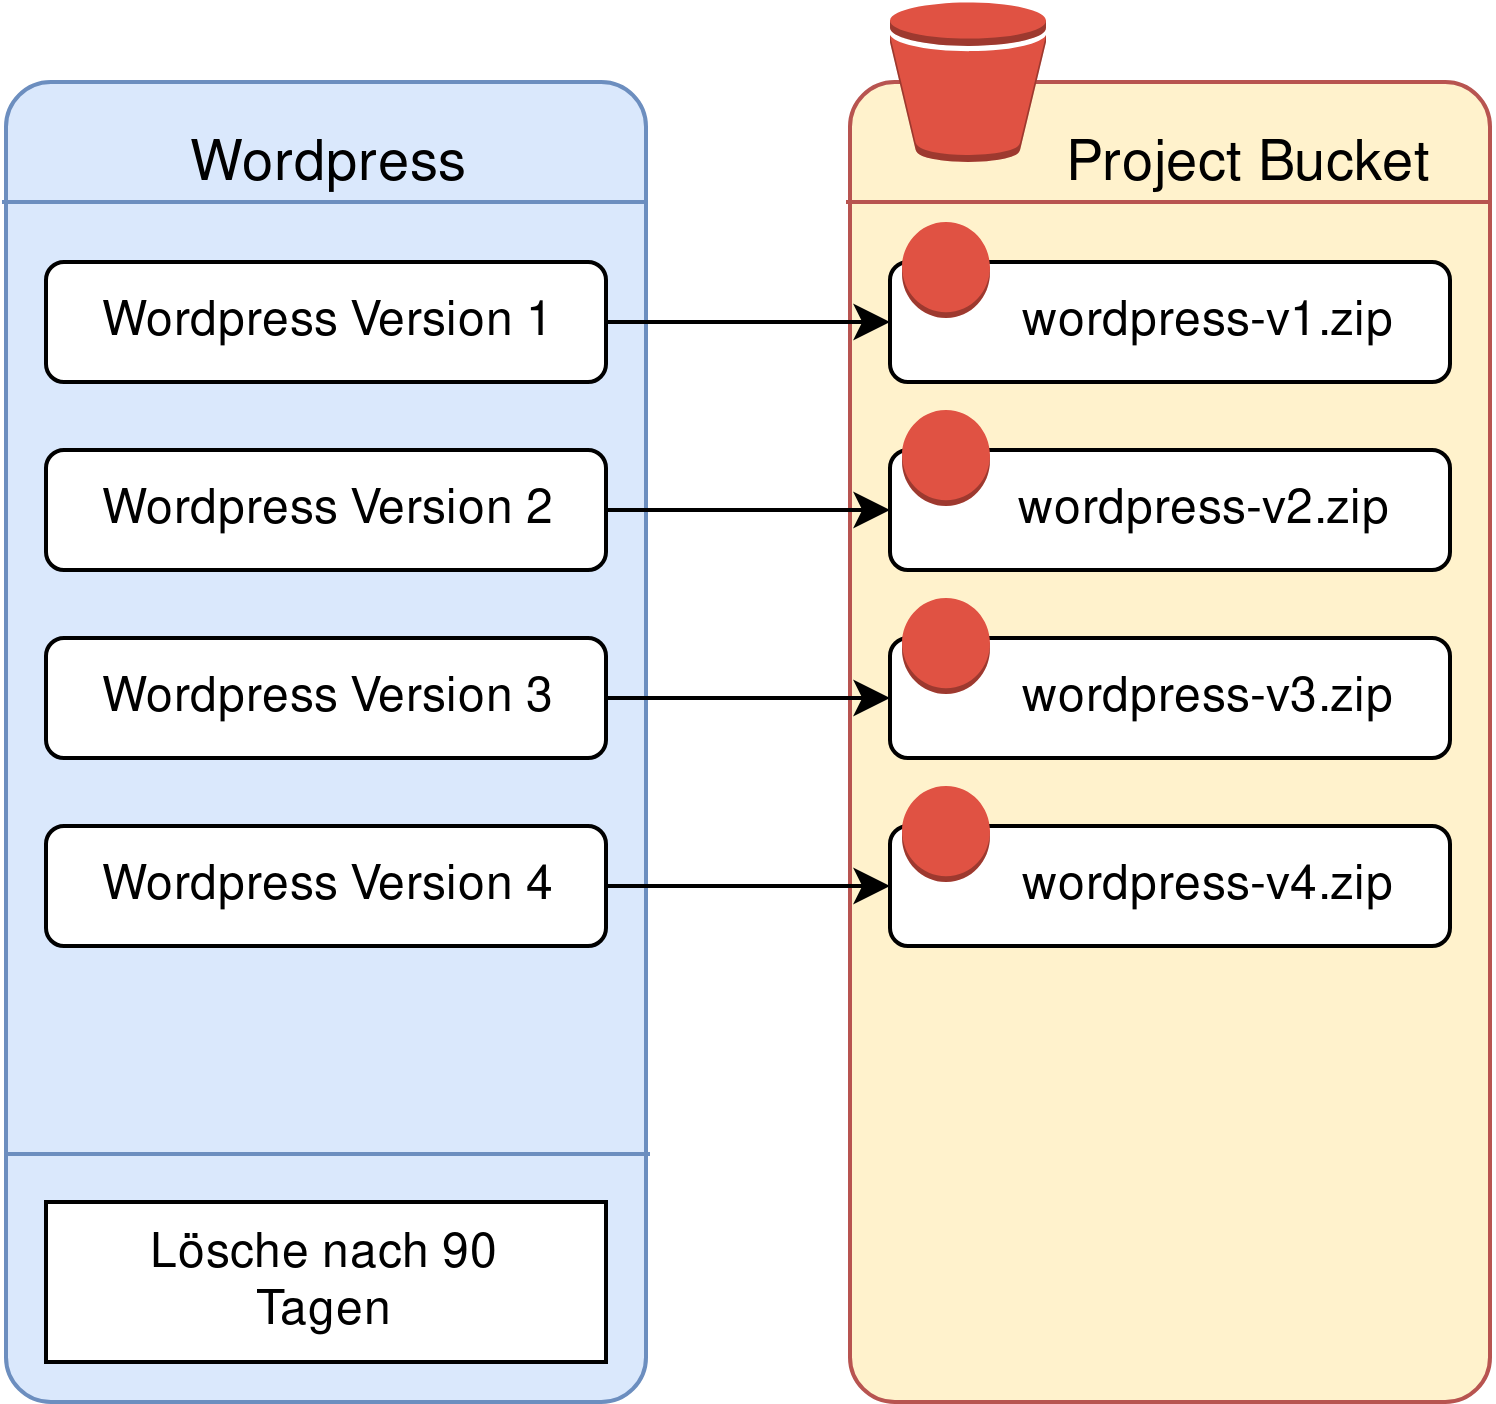
\includegraphics[height=5.5cm]{applicationversion}
  \end{flushright}
  \end{column}
  \end{columns}
\end{frame}

\begin{frame}
  \frametitle{Die Environment}
  \framesubtitle{AWS::ElasticBeanstalk::Environment}
  \begin{itemize}
  \item<2-> Zentrale Resource des Deployments
  \item<3-> Erstellt und verwaltet einen Cloudformation Stack
  \item<4-> Verbindet:
    \begin{itemize}
    \item<4-> Application Version
    \item<5-> Environment Tier
      \begin{itemize}
      \item Bestimmt aus welchen Resourcen der Cloudformation Stack besteht
      \item z.Z. WebServer oder Worker
      \end{itemize}
    \item<6-> Platform 
      \begin{itemize}
      \item Spezielles AMI, das auf den Instanzen der zentralen Autoscaling Group der Environment läuft
      \item Wird auch Solution Stack genannt
      \item z.B. PHP, Python, Docker, Java ...
      \end{itemize}
    \item<7-> Configuration Options
    \end{itemize}
  \end{itemize}
\end{frame}


\section{Konfiguration}
\subsection{}

\begin{frame}
  \frametitle{Configuration Options}
  \begin{itemize}
  \item<1-> Hauptweg um die festen Bestandteile einer Environment anzupassen.
  \item<2-> Bestehen aus Key-Value-Pairs in Namespaces, z.B.
  
  aws:elb:listener ListenerProtocol = HTTP
  \item<3-> Dinge, die sich über Configuration Options einstellen lassen:
    \begin{itemize}
    \item<4-> Das VPC in das Resourcen gesetzt werden
    \item<5-> Die Autoscaling Group ( Größe, Trigger, Instanztypen, EC2Keys u.s.w. )
    \item<6-> Individuelle Variablen, die an die Anwendung weiter gegeben werden ( bei PHP z.B. durch das \$\_SERVER Array )
    \item<7-> Der Loadbalancer
    \item<8-> Ob die Environment überhaupt einen Loadbalancer hat, oder SingleInstance sein soll
    \item<9-> \dots
    \end{itemize}
  \end{itemize}
\end{frame}

\begin{frame}
  \frametitle{.ebextensions}
  \framesubtitle{Konfigurationen an der ApplicationVersion}
  Wenn im Rootverzeichnis einer ApplicationVersion ein Directory mit dem Namen .ebextensions existiert, werden YAML- und JSON-Dateien für  die Konfiguration von Environments ausgelesen, wenn diese ApplicationVersion ausgerollt wird.
  
  \uncover<2->{Erlaubte Sektionen:}
  \begin{itemize}
  \item<3-> \texttt{option\_settings} Configuration Options
  \item<4-> \texttt{packages, groups, users, sources, files, commands, services}
  \item<5-> \texttt{container\_commands} Wie Commands aus AWS::Cloudformation::Init, aber werden ausgeführt nachdem der Rest der Anwendung ausgerollt wurde
  \item<6-> \texttt{Resources} Zusätzliche Cloudformation Resources die in der Environment erstellt werden. Auf in der Environment gesetzte Configuration Options kann mit \texttt{Fn::GetOptionSetting} zugegriffen werden.
  \end{itemize}
\end{frame}

\begin{frame}
  \frametitle{Die 4. Resource: Das Configuration Template}
  \framesubtitle{AWS::ElasticBeanstalk::ConfigurationTemplate}
  \begin{itemize}
  \item Speicherformat für Configuration Options
  \item<2-> Lässt sich einer Environment anhängen
  \item<3-> Kann auch die Platform für die Environment festlegen
  \item<4-> Kann zusätzlich zu eigenen Configuration Options auch bei der Erstellung Configuration Options aus einer bestehenden Environment oder einem anderen Configuration Template erben
  \end{itemize}
\end{frame}

\begin{frame}
  \frametitle{Configuration Option Precedence}
  \begin{center}
  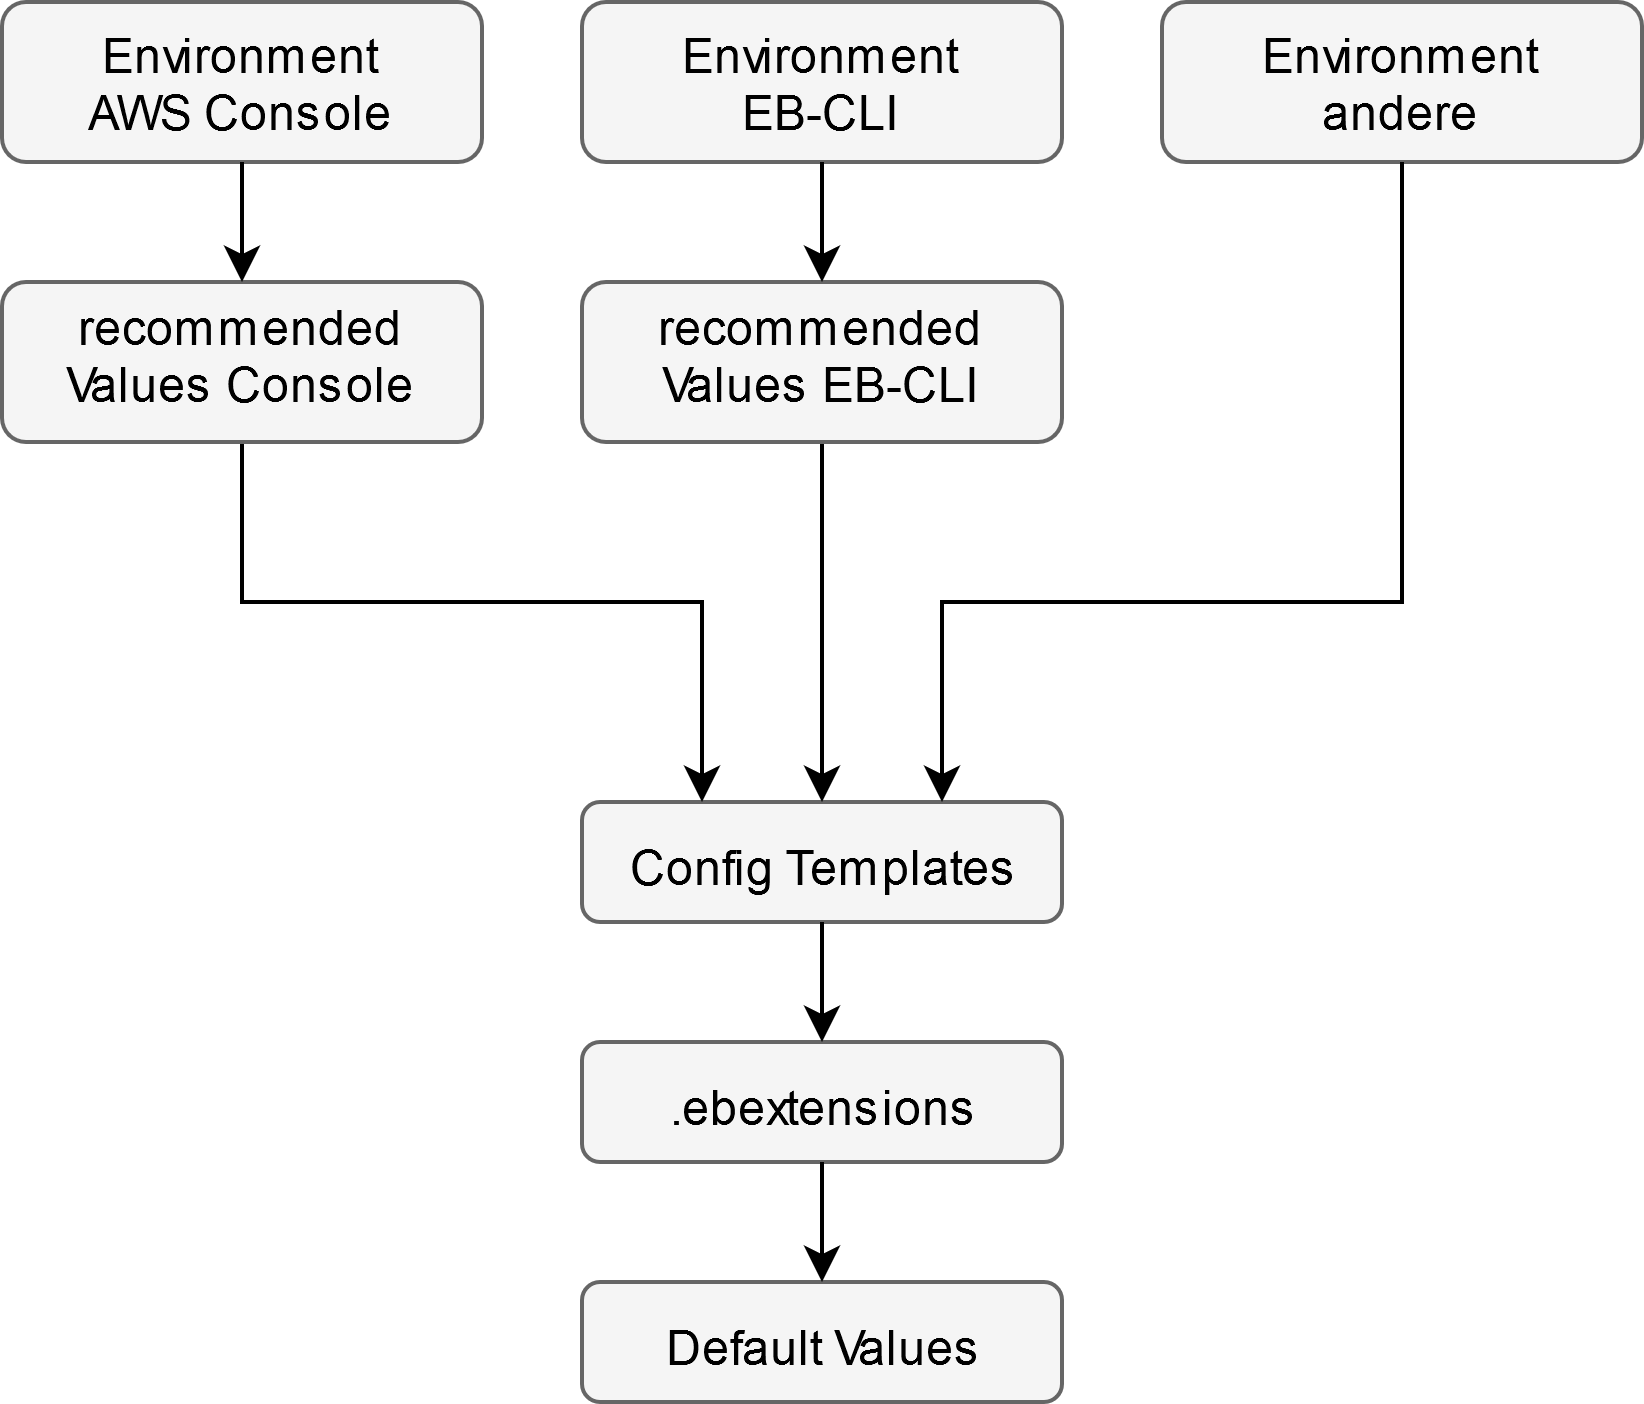
\includegraphics[height=6cm]{precedence}
  \end{center}
\end{frame}

\section{Praxis EB-CLI}
\subsection{}

\begin{frame}[fragile]
  \frametitle{Wordpress vorbereiten}
  \begin{lstlisting}[language=Bash]
  $ wget https://wordpress.org/latest.tar.gz
  $ tar -xvzf ./latest.tar.gz wordpress
  $ vim wordpress/wp-config.php
  \end{lstlisting}
\end{frame}

\begin{frame}[fragile]
  \frametitle{wp-config.php}
  \begin{lstlisting}[language=PHP]
<?php
define('DB_NAME', $_SERVER['RDS_DB_NAME']);
define('DB_USER', $_SERVER['RDS_USERNAME']);
define('DB_PASSWORD', $_SERVER['RDS_PASSWORD']);
define('DB_HOST', $_SERVER['RDS_HOSTNAME'] . ':' . $_SERVER['RDS_PORT']);
...
  \end{lstlisting}
\end{frame}

\begin{frame}[fragile]
  \frametitle{eb init}
  \begin{lstlisting}[language=Bash]
$ eb init

Select a default region
1) us-east-1 : US East (N. Virginia)
2) us-west-1 : US West (N. California)
3) us-west-2 : US West (Oregon)
4) eu-west-1 : EU (Ireland)
(default is 3): 4

Select an application to use
1) [ Create new Application ]
(default is 1): 1

Enter Application Name
(default is "wordpress"): wordpress
Application wordpress has been created.
  \end{lstlisting}
\end{frame}

\begin{frame}[fragile]
  \frametitle{eb create}
  \scriptsize
  \begin{lstlisting}[language=Bash]
$ eb create -db wordpress1
Enter an RDS DB username (default is "ebroot"):
Enter an RDS DB master password:
Creating application version archive "app-171102_151050".
Uploading: [##################################################] 100% Done...
--- Waiting for Application Versions to be pre-processed ---
Finished processing application version app-171102_151050
Environment details for: wordpress1
  Application name: wordpress
  Region: eu-west-1
  Deployed Version: app-171102_151050
  Environment ID: e-jgxsxns3dk
  Platform: arn:aws:eb:eu-west-1::platform/PHP 5.4 running on Amazon Linux/2.5.0
  Tier: WebServer-Standard
  CNAME: UNKNOWN
  Updated: 2017-11-02 15:11:00.901000+00:00
Printing Status:
INFO: createEnvironment is starting.
INFO: Using eb-eu-west-1-163962199350 as Amazon S3 bucket for environment data.
...
INFO: Environment health has transitioned from Pending to Ok. Initialization completed 2 seconds ago and took 9 minutes.
INFO: Successfully launched environment: wordpress1
  \end{lstlisting}
  \normalsize
\end{frame}

\begin{frame}
\frametitle{Ergebnisse}
  \begin{center}
  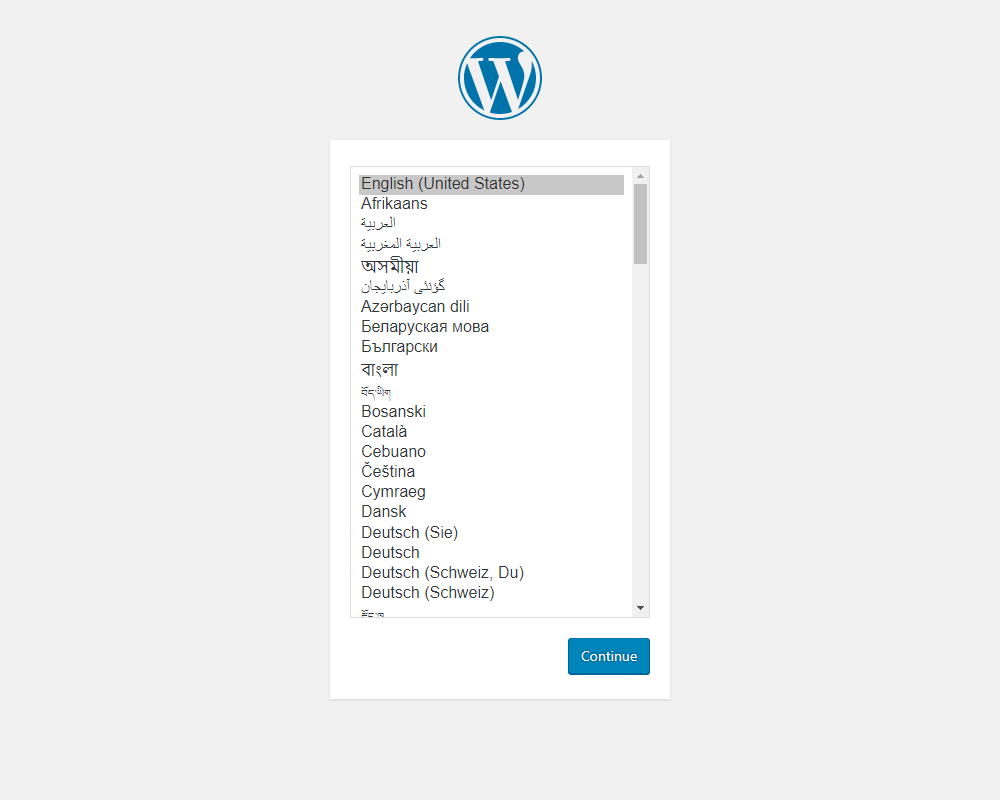
\includegraphics[height=7cm]{wordpress}
  \end{center}
\end{frame}

\begin{frame}
\frametitle{Ergebnisse!}
  \begin{center}
  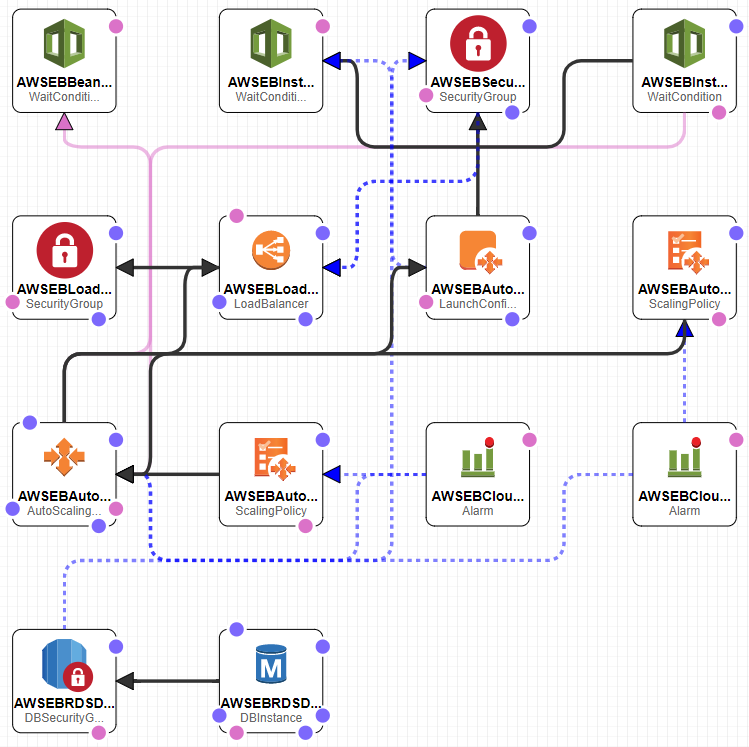
\includegraphics[height=7cm]{stack}
  \end{center}
\end{frame}

\section{Praxis Cloudformation}
\subsection{}

\begin{frame}
\frametitle{Die Datenbank: Down the rabbit hole}
  \begin{center}
  \texttt{eb create \only<1>{-db}\only<2->{{\huge -db}} wordpress1}
  
  \vspace{3mm}
  
  \uncover<2->{Wie haben sie das gemacht?}
  
  \vspace{3mm}
  
  \uncover<3->{Templates für Templates}
  \end{center}
\end{frame}

\begin{frame}
\frametitle{Probleme mit Cloudformation}
  Wir schreiben ein Cloudformation Template, \pause
  das einen Stack beschreibt, \pause
  das ein Werkzeug definiert, \pause
  das ein Cloudformation Template aus anderen Templates baut, \pause
  um die Resourcen zu definieren, auf denen unsere Applikation laufen soll.\pause
  
  \vspace{3mm}
  
  Application Versions sollen von Elastic Beanstalk selber verwaltet werden\pause , aber Cloudformation Stacks sind idempotent.\pause
  
  \vspace{3mm}
  
  Die anderen Elastic Beanstalk Resourcen haben unterschiedliche Lebenszyklen.
\end{frame}

\begin{frame}
  \frametitle{Ein Lösungsansatz}
  \begin{center}
  \begin{tabular}{ m{5.5cm} | m{5.5cm} }
  \uncover<2->{\textbf{Application Stack}

  Definiert:
  \begin{itemize}
  \item Application
  \item Dev Configuration Template
  \item Prod Configuration Template
  \end{itemize}
  Lebenszyklus: lang}
  \vspace{1mm}&
  \uncover<3->{\textbf{Dev Environment Stack}

  Definiert:
  \begin{itemize}
  \item VPC mit 2 Subnetzen
  \item Eine RDS Instanz
  \item Die Development Environment
  \end{itemize}
  Lebenszyklus: kurz}
  \vspace{1mm} \\
  \hline
  \rule{0pt}{2.6ex}
  \uncover<4->{\textbf{Prod Network Stack}

  Definiert:
  \begin{itemize}
  \item VPC mit 4 Subnetzen
  \item Multi-AZ RDS Instanz
  \end{itemize}
  Lebenszyklus: mittel} &
  \uncover<5->{\textbf{Prod Environment Stack}

  ( 2 Abhängigkeiten )

  Definiert:
  \begin{itemize}
  \item Die Production Environment
  \end{itemize}
  Lebenszyklus: kurz}
  \end{tabular}
  \end{center}
\end{frame}


\section{Schluss}
\subsection{}

\begin{frame}
  \frametitle{Dinge, die ich (bis jetzt) ausgelassen habe.}
  \begin{LARGE}
  \begin{addmargin}[20mm]{0mm}
  env.yaml\pause
  
  \vspace{5mm}  
  
  Environment Groups\pause
    
  \vspace{5mm}  
  
  Custom Platforms \pause ( Packer Templates )
  \end{addmargin}
  \end{LARGE}
\end{frame}

\begin{frame}
  \frametitle{Ein Wort der Warnung}
  \uncover<2->{{\large Dinge haben mehrere Namen}}
  \begin{itemize}
  \item<3-> Configuration Template = Saved Configuration
  \item<4-> Environment Tier/Type
  \item<4-> Solution Stack = !(Custom) Platform
  \item<4-> (Application) Version Lifecycle Config / (Application) Resource Lifecycle Config / Lifecycle Policy
  \end{itemize}
  
  \vspace{8mm}
  
  \uncover<5->{{\large Es gibt für alles eine Ausnahme}}
\end{frame}

\begin{frame}
  \begin{center}
  \Huge
  Fazit
  \end{center}
\end{frame}

\end{document}